\providecommand{\main}{../../..}
\documentclass[\main/dresen_thesis.tex]{subfiles}
  \renewcommand{\thisPath}{\main/chapters/theoreticalBackground/ferrites}
\begin{document}

  \section{Iron Spinels}
  In this work, nanoparticles are prepared chemically from iron and cobalt salts for the study of ordered magnetic structures on the nanoscale.
  Iron is the fourth most common element in the Earth's crust and ferromagnetic at room temperature in its elemental state.
  Typically, the elements are rarely found in their native state but they tend to oxidize and form compounds with oxygen \cite{Parkinson_2016_Irono}.
  In the iron oxides, the oxygen anions \ch{O^{2-}} form a close packed lattice with octahedral and tetrahedral interstices as shown in \reffig{fig:theoreticalBackground:ferrites:ironOxides}.
  \begin{figure}[b]
    \centering
    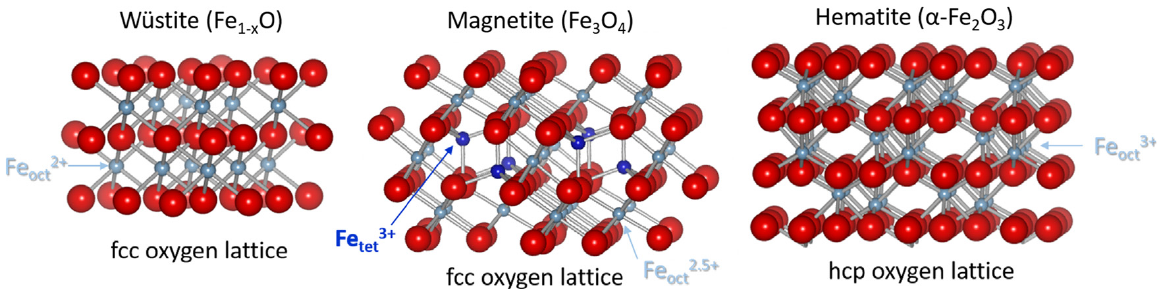
\includegraphics[width=\textwidth]{ferrites_iron_oxides_structures}
    \caption{\label{fig:theoreticalBackground:ferrites:ironOxides}Iron oxide structures. The red spheres represent the close packed \ch{O^{2-}} lattice and the iron cations occupy either the tetrahedral or octahedral interstices, where different configurations with different oxidation states result in the various compounds. Image taken from  \cite{Parkinson_2016_Irono}.}
  \end{figure}

  When both $\ch{Fe^{2+}}$ and $\ch{Fe^{3+}}$ are present, magnetite forms as the stable phase with the structure of an inverse spinel.
  The inverse spinel structure of a compound \ch{AB2O4} is commonly noted as \ch{(A)[BA]O4}, where the round bracket notes the atoms in the tetrahedral and the square bracket the atoms in the octahedral position.
  In magnetite (\ch{Fe3O4}), the tetrahedral sites are occupied by $\ch{Fe^{3+}}$ and the octahedral sites 1:1 by $\ch{Fe^{2+}}$ and $\ch{Fe^{3+}}$, which is noted by (\ch{Fe^{3+}})[\ch{Fe^{2+}Fe^{3+}}]$\ch{O4}$. When magnetite is oxidates at low temperatures, maghemite ($\gamma-\ch{Fe2O3}$) forms which is a a defective inverse spinel only composed of $\ch{Fe^{3+}}$ and additional vacancies in the octahedral sites to ensure charge neutrality, noted by $(\ch{Fe^{3+}})[\ch{Fe^{3+}}_{5/3}\square_{1/3}]\ch{O4}$.
  Magnetite and maghemite are both ferrimagnetic at room temperature due to the antiferromagnetic coupling between the trivalent cations on the tetrahedral and octahedral sites.
  To large parts the magnetism of the compound can therefore be understood by considering the electronic configuration of the surplus atoms on the octahedral site, which will be discussed in the following subsections for maghemite, magnetite and the case when bivalent cobalt cations $\ch{Co^{2+}}$ are substituted for iron.

  It is noteworthy that maghemite is a metastable iron oxide state.
  For fully oxidized iron upon exposure to elevated temperatures, the compound transitions to hematite with the oxygen anions on a hcp lattice and  all $\ch{Fe^{3+}}$ on octahedral sites.
  Hematite is only weakly ferromagnetic at room temperature and antiferromagnetic below $T \eq 260 \unit{K}$.
  On the other side of the spectrum, in a strongly reducing environment with only $\ch{Fe^{2+}}$ present, w\"ustite (\ch{Fe_{1-x}O}) is the stable phase, which crystallizes typically in a defective rocksalt structure where oxygen forms an fcc lattice and deficient \ch{Fe^{2+}} occupies the octahedral sites.
  W\"ustite is paramagnetic at room temperature and antiferromagnetic at temperatures below $T_N \approx 203 K$.

  \subfile{\thisPath/maghemite/maghemite}
  \subfile{\thisPath/cobaltferrite/cobaltferrite}

\end{document}